%%%%%%%%%%%%%%%%%%%%%%%%%%%%%%%%%%%%%%%%%%%%%%%%%%%%%%%%%%%%%%%%%%%%%%%%%%%%%%%%
% Template for USENIX papers.
%
% History:
%
% - TEMPLATE for USENIX papers, specifically to meet requirements of
%   USENIX '05. originally a template for producing IEEE-format
%   articles using LaTeX. written by Matthew Ward, CS Department,
%   Worcester Polytechnic Institute. adapted by David Beazley for his
%   excellent SWIG paper in Proceedings, Tcl 96. turned into a
%   smartass generic template by De Clarke, with thanks to both the
%   above pioneers. Use at your own risk. Complaints to /dev/null.
%   Make it two column with no page numbering, default is 10 point.
%
% - Munged by Fred Douglis <douglis@research.att.com> 10/97 to
%   separate the .sty file from the LaTeX source template, so that
%   people can more easily include the .sty file into an existing
%   document. Also changed to more closely follow the style guidelines
%   as represented by the Word sample file.
%
% - Note that since 2010, USENIX does not require endnotes. If you
%   want foot of page notes, don't include the endnotes package in the
%   usepackage command, below.
% - This version uses the latex2e styles, not the very ancient 2.09
%   stuff.
%
% - Updated July 2018: Text block size changed from 6.5" to 7"
%
% - Updated Dec 2018 for ATC'19:
%
%   * Revised text to pass HotCRP's auto-formatting check, with
%     hotcrp.settings.submission_form.body_font_size=10pt, and
%     hotcrp.settings.submission_form.line_height=12pt
%
%   * Switched from \endnote-s to \footnote-s to match Usenix's policy.
%
%   * \section* => \begin{abstract} ... \end{abstract}
%
%   * Make template self-contained in terms of bibtex entries, to allow
%     this file to be compiled. (And changing refs style to 'plain'.)
%
%   * Make template self-contained in terms of figures, to
%     allow this file to be compiled. 
%
%   * Added packages for hyperref, embedding fonts, and improving
%     appearance.
%   
%   * Removed outdated text.
%
%%%%%%%%%%%%%%%%%%%%%%%%%%%%%%%%%%%%%%%%%%%%%%%%%%%%%%%%%%%%%%%%%%%%%%%%%%%%%%%%

\documentclass[letterpaper,twocolumn,10pt]{article}
\usepackage{styles}

% to be able to draw some self-contained figs
\usepackage{tikz}
\usepackage{amsmath}

% inlined bib file
\usepackage{filecontents}

%-------------------------------------------------------------------------------
\begin{filecontents}{\jobname.bib}
%-------------------------------------------------------------------------------
@Book{arpachiDusseau18:osbook,
  author =       {Arpaci-Dusseau, Remzi H. and Arpaci-Dusseau Andrea C.},
  title =        {Operating Systems: Three Easy Pieces},
  publisher =    {Arpaci-Dusseau Books, LLC},
  year =         2015,
  edition =      {1.00},
  note =         {\url{http://pages.cs.wisc.edu/~remzi/OSTEP/}}
}
@InProceedings{waldspurger02,
  author =       {Waldspurger, Carl A.},
  title =        {Memory resource management in {VMware ESX} server},
  booktitle =    {USENIX Symposium on Operating System Design and
                  Implementation (OSDI)},
  year =         2002,
  pages =        {181--194},
  note =         {\url{https://www.usenix.org/legacy/event/osdi02/tech/waldspurger/waldspurger.pdf}}}
\end{filecontents}

%-------------------------------------------------------------------------------
\begin{document}
%-------------------------------------------------------------------------------

%don't want date printed
\date{}

% make title bold and 14 pt. font (Latex default is non-bold, 16 pt.)
\title{\Large \bf Proxy Herd with Python 3.9.2's \texttt{asyncio}}

\maketitle

%-------------------------------------------------------------------------------
\begin{abstract}
%-------------------------------------------------------------------------------
This research was conducted in order to determine if Python's \texttt{asyncio} 
library is viable for implementing an application server herd. Using a local
prototype to investigate the pros and cons of \texttt{asyncio}, application
performance and usability were analyzed and compared to Java and Node.js
counterparts. After consideration, it has been determined that \texttt{asyncio} 
is a perfectly reasonable framework to use to develop an application server 
herd.
\end{abstract}

%-------------------------------------------------------------------------------
\section{Introduction}
%-------------------------------------------------------------------------------
\par
Wikipedia-style platforms are implemented on the Wikimedia server platform, a
stack consisting of Debian GNU/Linux, Apache, Memcached, MariaDB, Elasticsearch,
Swift, PHP + JavaScript, and redundant web servers. 

\subsection{Motivation}
\par
The Wikimedia server platform works fine for Wikipedia, however, if a new
service is created that updates more frequently, requires more flexibility in
protocols, and is tailored towards more mobile clients, the PHP + JavaScript in
the existing server platform may throttle performance. As a result, this new
application may favor being built on an application server herd architecture.
This architecture centers around the servers' ability to communicate with one
another, as well as communicating with the core database. These additional
connections make the server herd very efficient in handling volatile data, as
new data can be propagated between each server, removing the need for constant
communication with the core database, making this architecture perfect for this
hypothetical platform. This shift in architecture requires that an appropriate
framework be found for it to be built on, which prompts the investigation into
\texttt{asyncio}, a Python library allowing for the development of single-
threaded, event-driven, concurrent code.

\subsection{Server-side Prototyping}
\par
In order to better understand whether \texttt{asyncio} is viable for the
purposes of this application, a small prototype was implemented, consisting of 5
servers: Riley, Jaquez, Juzang, Campbell, and Bernard. Each of these servers is
capable of accepting TCP connections from clients, and was hosted locally on
a set of 5 different ports. These servers were run using source code written in
the file \texttt{server.py}, started by the \texttt{asyncio.run()} subroutine.
These servers communicate bidirectionally, where Riley talks to Jaquez and
Juzang, Bernard talks with Jaquez, Juzang, and Campbell, and Juzang talks with
Campbell. This pattern allows a single request to any server to be propagated to
each other server using a flooding algorithm built on AT messages and the
\texttt{asyncio.open\_connection()} subroutine. AT messages consist of the
origin server's name, a time difference between sending and receiving, the
domain name of the client, the client's geolocation, and a timestamp for when
the message was sent. Each server is then responsible for processing AT
messages and updating their client information appropriately to prevent
infinite propagation loops. Every action these servers take is logged in a file,
along with the timestamp that the action was performed at.

\subsection{Client-side Prototyping}
\par
Each of the 5 servers may accept 1 of 2 messages from clients that are connected
to them. The first of these messages is the IAMAT message, where the client 
provides a domain name, latitude and longitude, and a timestamp of when the
message was sent. Upon receiving an IAMAT message, servers will propagate the
location of the client to every other server using the flooding algorithm
detailed above. This will then be followed by a response to the client in the
same form as the AT message that the servers use to keep themselves updated.
The other message is a WHATSAT message, where the client provides a domain name,
a radius below 50 km, and a bound on the amount of information they want to 
access. This will cause a server to initiate a call to the Google Places API,
using the information provided in the message. This call to the API provides
the server with location information in the form of JSON object, which is then
returned to the user, following another AT message. Any message that the client
sends that does not fall within these guidelines is replied to with an error
message.

%-------------------------------------------------------------------------------
\section{Python vs. Java}
%-------------------------------------------------------------------------------
\par

\subsection{Type Checking}
\par

\subsection{Memory Management}
\par

\subsection{Multithreading}
\par

%-------------------------------------------------------------------------------
\section{\texttt{asyncio} vs. Node.js}
%-------------------------------------------------------------------------------
\par

%-------------------------------------------------------------------------------
\section{Conclusions}
%-------------------------------------------------------------------------------
\par

\subsection{Ease of Use}

\subsection{Performance Implications}

\subsection{Features of Python 3.9+}

\subsection{Problems Encountered}

\subsection{Evaluation}

%-------------------------------------------------------------------------------
\section{References}
%-------------------------------------------------------------------------------
"asyncio Source Code"
Updated December 18, 2020
Available: \\ https://github.com/python/cpython/tree/master/Lib/asyncio \\
\\
"asyncio - Asynchronous I/O" 
Updated March 6, 2021.
Available: \\ https://docs.python.org/3/library/asyncio.html \\
\\
P. Eggert "Project. proxy herd with asyncio" 
Updated February 24, 2021. 
Available: \\ https://web.cs.ucla.edu/classes/winter21/cs131/hw/pr.html \\
\\
"What's New In Python 3.9"
Updated March 6, 2021.
Available: \\ https://docs.python.org/3/whatsnew/3.9.html


%%%%%%%%%%%%%%%%%%%%%%%%%%%%%%%%%%%%%%%%%%%%%%%%%%%%%%%%%%%%%%%%%%%%%%%%%%%%%%%%
\end{document}
%%%%%%%%%%%%%%%%%%%%%%%%%%%%%%%%%%%%%%%%%%%%%%%%%%%%%%%%%%%%%%%%%%%%%%%%%%%%%%%%

%%  LocalWords:  endnotes includegraphics fread ptr nobj noindent
%%  LocalWords:  pdflatex acks

% \begin{figure}
%   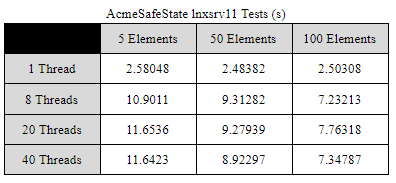
\includegraphics[scale=0.8]{acmesafe-11.png}
%   \caption{\label{fig:vectors} Table of total time results from testing AcmeSafeState on lnxsrv11, measured in seconds. }
% \end{figure}